%%
%% Automatically generated file from DocOnce source
%% (https://github.com/hplgit/doconce/)
%%

% #define PREAMBLE

% #ifdef PREAMBLE
%-------------------- begin preamble ----------------------

\documentclass[%
oneside,                 % oneside: electronic viewing, twoside: printing
final,                   % draft: marks overfull hboxes, figures with paths
10pt]{article}

\listfiles               % print all files needed to compile this document

\usepackage{relsize,makeidx,color,setspace,amsmath,amsfonts,amssymb}
\usepackage[table]{xcolor}
\usepackage{bm,microtype}

\usepackage[pdftex]{graphicx}

% Packages for typesetting blocks of computer code
\usepackage{fancyvrb,framed,moreverb}

% Define colors
\definecolor{orange}{cmyk}{0,0.4,0.8,0.2}
\definecolor{tucorange}{rgb}{1.0,0.64,0}
\definecolor{darkorange}{rgb}{.71,0.21,0.01}
\definecolor{darkgreen}{rgb}{.12,.54,.11}
\definecolor{myteal}{rgb}{.26, .44, .56}
\definecolor{gray}{gray}{0.45}
\definecolor{mediumgray}{gray}{.8}
\definecolor{lightgray}{gray}{.95}
\definecolor{brown}{rgb}{0.54,0.27,0.07}
\definecolor{purple}{rgb}{0.5,0.0,0.5}
\definecolor{darkgray}{gray}{0.25}
\definecolor{darkblue}{rgb}{0,0.08,0.45}
\definecolor{darkblue2}{rgb}{0,0,0.8}
\definecolor{lightred}{rgb}{1.0,0.39,0.28}
\definecolor{lightgreen}{rgb}{0.48,0.99,0.0}
\definecolor{lightblue}{rgb}{0.53,0.81,0.92}
\definecolor{lightblue2}{rgb}{0.3,0.3,1.0}
\definecolor{lightpurple}{rgb}{0.87,0.63,0.87}
\definecolor{lightcyan}{rgb}{0.5,1.0,0.83}

\colorlet{comment_green}{green!50!black}
\colorlet{string_red}{red!60!black}
\colorlet{keyword_pink}{magenta!70!black}
\colorlet{indendifier_green}{green!70!white}

% Backgrounds for code
\definecolor{cbg_gray}{rgb}{.95, .95, .95}
\definecolor{bar_gray}{rgb}{.92, .92, .92}

\definecolor{cbg_yellowgray}{rgb}{.95, .95, .85}
\definecolor{bar_yellowgray}{rgb}{.95, .95, .65}

\colorlet{cbg_yellow2}{yellow!10}
\colorlet{bar_yellow2}{yellow!20}

\definecolor{cbg_yellow1}{rgb}{.98, .98, 0.8}
\definecolor{bar_yellow1}{rgb}{.98, .98, 0.4}

\definecolor{cbg_red1}{rgb}{1, 0.85, 0.85}
\definecolor{bar_red1}{rgb}{1, 0.75, 0.85}

\definecolor{cbg_blue1}{rgb}{0.87843, 0.95686, 1.0}
\definecolor{bar_blue1}{rgb}{0.7,     0.95686, 1}


\usepackage[T1]{fontenc}
%\usepackage[latin1]{inputenc}
\usepackage{ucs}
\usepackage[utf8x]{inputenc}

\usepackage{lmodern}         % Latin Modern fonts derived from Computer Modern

% Hyperlinks in PDF:

\usepackage{hyperref}
\hypersetup{
    breaklinks=true,
    colorlinks=true,
    linkcolor=seccolor,
    urlcolor=seccolor,
    citecolor=black,
    filecolor=black,
    %filecolor=blue,
    pdfmenubar=true,
    pdftoolbar=true,
    bookmarksdepth=3   % Uncomment (and tweak) for PDF bookmarks with more levels than the TOC
    }
%\hyperbaseurl{}   % hyperlinks are relative to this root

\setcounter{tocdepth}{2}  % number chapter, section, subsection

% Tricks for having figures close to where they are defined:
% 1. define less restrictive rules for where to put figures
\setcounter{topnumber}{2}
\setcounter{bottomnumber}{2}
\setcounter{totalnumber}{4}
\renewcommand{\topfraction}{0.95}
\renewcommand{\bottomfraction}{0.95}
\renewcommand{\textfraction}{0}
\renewcommand{\floatpagefraction}{0.75}
% floatpagefraction must always be less than topfraction!
% 2. ensure all figures are flushed before next section
\usepackage[section]{placeins}
% 3. enable begin{figure}[H] (often leads to ugly pagebreaks)
%\usepackage{float}\restylefloat{figure}

% prevent orhpans and widows
\clubpenalty = 10000
\widowpenalty = 10000

% http://www.ctex.org/documents/packages/layout/titlesec.pdf
\usepackage{titlesec}  % needed for colored section headings
%\usepackage[compact]{titlesec}  % reduce the spacing around section headings

% --- section/subsection headings with blue color ---
\definecolor{seccolor}{cmyk}{.9,.5,0,.35}  % siamltexmm.sty section color
\titleformat{name=\section}
{\color{seccolor}\normalfont\Large\bfseries}
{\color{seccolor}\thesection}{1em}{}
\titleformat{name=\subsection}
{\color{seccolor}\normalfont\large\bfseries}
{\color{seccolor}\thesubsection}{1em}{}
\titleformat{name=\paragraph}[runin]
{\color{seccolor}\normalfont\normalsize\bfseries}
{}{}{\indent}


% --- color every two table rows ---
\let\oldtabular\tabular
\let\endoldtabular\endtabular
\definecolor{appleblue}{rgb}{0.93,0.95,1.0}  % Apple blue
\renewenvironment{tabular}{\rowcolors{2}{white}{appleblue}%
\oldtabular}{\endoldtabular}


% --- end of standard preamble for documents ---

%\usepackage{flafter}

% makes figures appear closer to the defined location
\usepackage{float}
\floatplacement{figure}{H}


%%%% sets margins
\usepackage[letterpaper, portrait, margin=0.5in]{geometry}

% insert custom LaTeX commands...

\raggedbottom
\makeindex

%-------------------- end preamble ----------------------

\begin{document}

% endif for #ifdef PREAMBLE
% #endif


% ------------------- main content ----------------------



% ----------------- title -------------------------

\title{{\color{seccolor} Getting Started with Python in Engineering}}

% ----------------- author(s) -------------------------

\author{Neal Gordon}

% ----------------- end author(s) -------------------------

\date{Feb 20, 2017}
\maketitle

% inline figure
\centerline{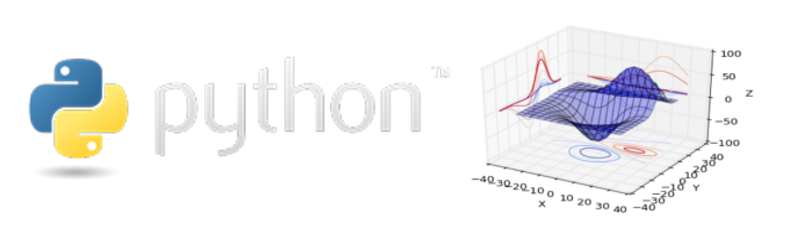
\includegraphics[width=0.9\linewidth]{fig/pythonengineering.png}}



% !split
\subsection{Summary}

\begin{itemize}
\item Why python

\item Installation

\item Help and Documentation

\item Python Syntax
\begin{itemize}

 \item Comments and Strings

 \item Printing

 \item Variables and Datatypes

 \item Lists and Arrays

 \item Indentation and Conditionals

 \item Loops

 \item Functions

 \item Modules

\end{itemize}

\noindent
\item Numerical Python
\begin{itemize}

 \item Arrays

 \item Logical Indexing

 \item Multi-Dimensional Arrays (matrices)

 \item Plotting

\end{itemize}

\noindent
\item References and Links
\end{itemize}

\noindent
% !split
\subsection{Why code}

It's just another tool to solve engineering problems

% !bpop
\begin{itemize}
 \item Hand calculations are by far the best way to start solving a problem, but not always the best way to find the solution you need.

 \item Spreadsheets are a great mix of a database and calculator, but not great at either

 \item Databases are the best way to store data, but typically are interfaced with code

 \item The best calculators are the ones that work out of the box, but are also 100\% customizable

 \item diversify skills other than just basic data entry or calculations, such as web design and development, software development, CAD/CAE API development

 \item Automate the boring parts of your job with code so you can enjoy the awesome parts
\end{itemize}

\noindent
% !epop

% !split
\subsection{Why python}



% inline figure
\centerline{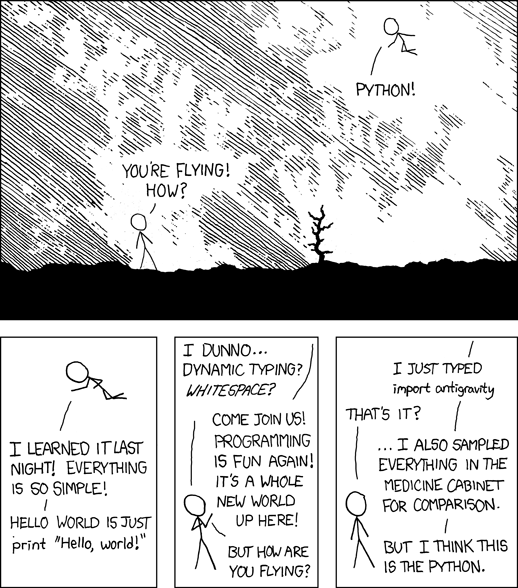
\includegraphics[width=0.9\linewidth]{fig/xkcd-python.png}}



% !split
\subsection{Why python}

Python is a general purpose programming language, and is used in web development, graphical user interfaces, IT automation, and SCIENTIFIC COMPUTING



% inline figure
\centerline{
\includegraphics[width=0.75\linewidth]{fig/pythonapps.png}}



% !split
\subsection{Python vs Matlab}

Matlab is a powerful scientific computing language and software development package that is superior for many mathematical operations, specifically linear algebra, signal processing, and modeling dynamic systems(via Simulink). However, for many engineering applications is not worth the cost. Although many of the Matlab libraries  may be arguably better than comparable python libraries, they are closed source and cannot be modified or inspected by users. Also, sharing code with collaborators or publications requires other users to have licenses.

Python, on the other hand, is a general programming language so it is very good at many tasks, but was not designed exclusively for scientific computing



% inline figure
\centerline{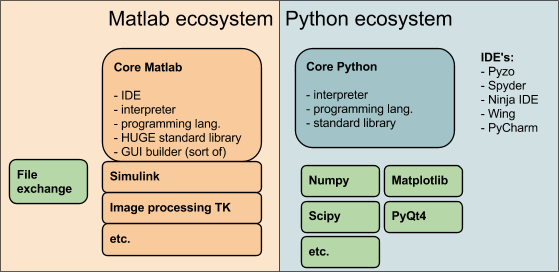
\includegraphics[width=1.0\linewidth]{fig/pythonvsmatlab.png}}




% !split
\subsection{Python vs Matlab}

\textbf{Python Positives}
\begin{itemize}
\item being easy and fun to learn with great online forumns and open communities

\item many libraries for scientific computing, server and desktop management and automation

\item works great on Linux, Mac and Windows and easily integrates with other languages (fortran, C, java)

\item scripts are easily integrated with other applications

\item FREE, open-source and customizable. Every module/library can be modified
\end{itemize}

\noindent
\textbf{Matlab Positives}
\begin{itemize}
\item professional technical support

\item fast(er) execution

\item being straightforward for simple scientific calculations
\end{itemize}

\noindent
% !split
\subsection{Installation}

To get started, choose the python distribution you want. I would recommend anaconda, which has most of the scientific packages that are needed in one installation, but more importantly, comes with a package manager called \texttt{conda}, which is a big help when installing and updating python packages (especially on Windows) and \href{{http://conda.pydata.org/docs/using/envs.html}}{managing environments} if we want to use multiple versions of python.

\begin{itemize}
\item \href{{https://www.continuum.io/downloads#34}}{Anaconda} or \href{{http://conda.pydata.org/miniconda.html}}{Miniconda} for Linux, Mac, and Windows

\item \href{{http://www.pyzo.org/index.html}}{pyzo} For Linux, Mac, and Windows

\item \href{{http://winpython.sourceforge.net/}}{winpython} for Windows

\item \href{{http://python-xy.github.io/}}{python(x,y)} for Windows
\end{itemize}

\noindent
Installing new packages and updating is easy. \texttt{conda} takes care of dependencies and version compatibility.

\begin{Verbatim}[numbers=none,fontsize=\fontsize{9pt}{9pt},baselinestretch=0.95,xleftmargin=2mm]
# install a single library
conda install numpy

# update a single library
conda update numpy

# update all packages
conda update --all
\end{Verbatim}


% !split
\subsection{A Note on Versions}

Python currently has 2 popular versions, 2x and 3x. 2x has a lot of legacy code still in use, but support is being phased out. Either version works, but I would recommend always trying to default to the latest release (v3.5).

Among many major changes, the two changes I find most troublesome is the print command and division.


\textbf{print changes}
\begin{Verbatim}[numbers=none,fontsize=\fontsize{9pt}{9pt},baselinestretch=0.95,xleftmargin=2mm]
# v2.7
print "hello world"  # hello world

# v3.5
print("hello world")  # hello world
\end{Verbatim}


\textbf{division changes}
\begin{Verbatim}[numbers=none,fontsize=\fontsize{9pt}{9pt},baselinestretch=0.95,xleftmargin=2mm]
#v2.7
7 / 4
# 1
7 / 4.0
# 1.75
7 // 4
# 1

#v3.5
7 / 4
# 1.75
7 // 4
# 1
\end{Verbatim}

% !split
\subsection{Development Environments}

Python has many options for programming, and graphical user interface development. Many different integrated development environments (IDE), such as spyder. Although not a polished, spyder is similar to the Matlab interface. Browser based jupyter notebooks are a great way to write web-ready content or sharing calculations or plots



% inline figure
\centerline{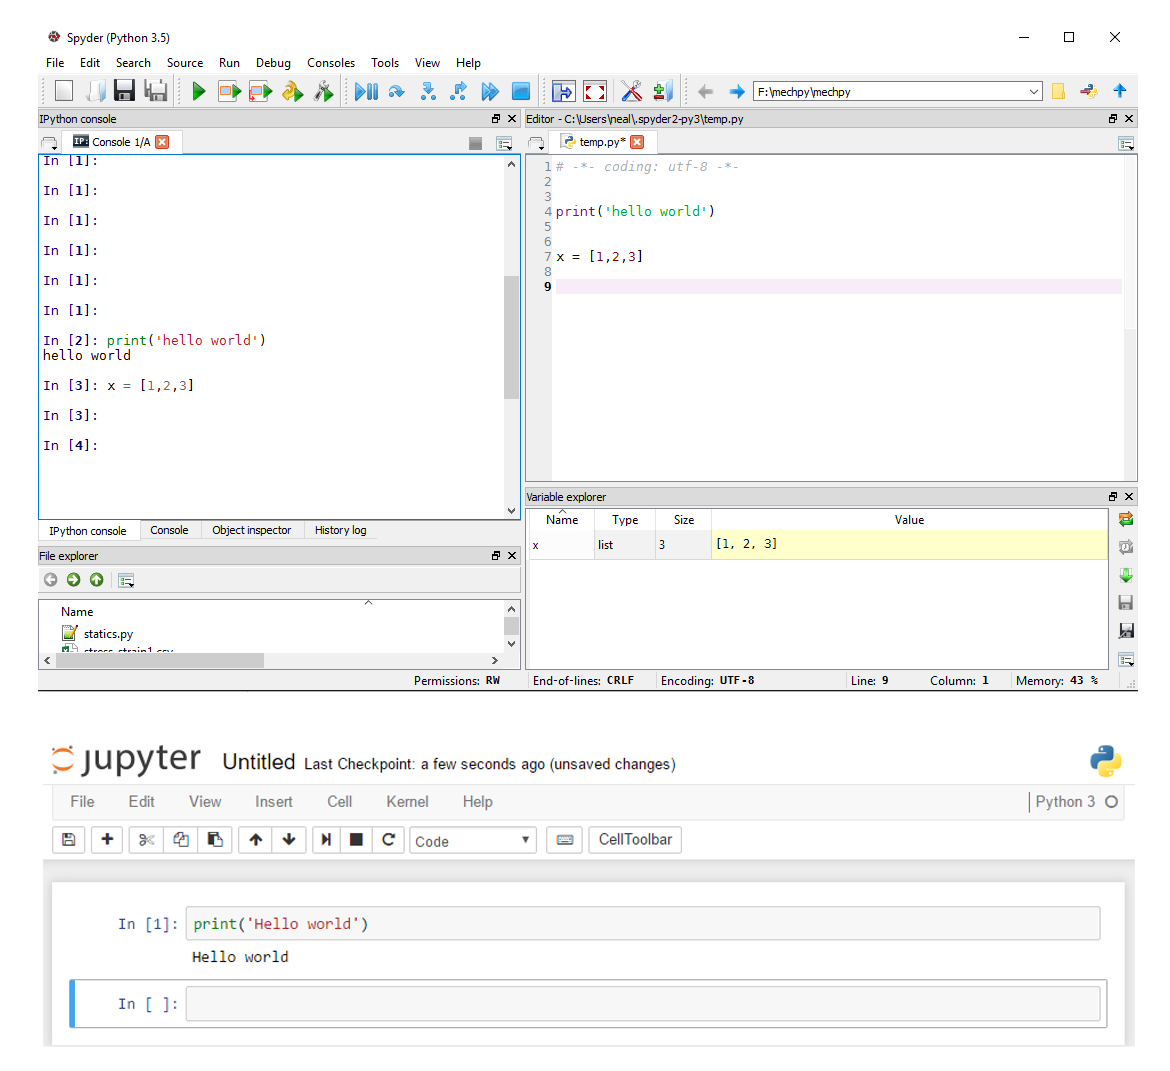
\includegraphics[width=0.9\linewidth]{fig/jupyterspyder.png}}




% !split
\subsection{First Program}

Before we go any further, let's put together a simple python script and run it. First, open a text file and type

\begin{Verbatim}[numbers=none,fontsize=\fontsize{9pt}{9pt},baselinestretch=0.95,xleftmargin=2mm]
print('hello world')
\end{Verbatim}

save it as \texttt{hello.py}. Now, lets open a command window. In windows, my preferred way is to shift+right-click in a window and select \textbf{open in terminal}. The other option is to run \texttt{cmd} from the start menu. Type the following and hit enter.

\begin{Verbatim}[numbers=none,fontsize=\fontsize{9pt}{9pt},baselinestretch=0.95,xleftmargin=2mm]
python hello.py
\end{Verbatim}

% !bpop
\begin{Verbatim}[numbers=none,fontsize=\fontsize{9pt}{9pt},baselinestretch=0.95,xleftmargin=2mm]
hello world
\end{Verbatim}
% !epop

You should have seen your print statement printed to the console. If so, congratulations!, you have executed your first python program. Some other ways to run your program are through the ipython interpreter, which can be launched from your command line by running \texttt{ipython} or using the ipython install shortcut

\begin{Verbatim}[numbers=none,fontsize=\fontsize{9pt}{9pt},baselinestretch=0.95,xleftmargin=2mm]
In [1]: run hello.py
\end{Verbatim}

% !bpop
\begin{Verbatim}[numbers=none,fontsize=\fontsize{9pt}{9pt},baselinestretch=0.95,xleftmargin=2mm]
hello world
\end{Verbatim}
% !epop


% !split
\subsection{Help and Documentation}

if help is ever needed, for example of the math module, in the ipython console, type

\begin{Verbatim}[numbers=none,fontsize=\fontsize{9pt}{9pt},baselinestretch=0.95,xleftmargin=2mm]
help(print)
#or
print?
\end{Verbatim}

% !bpop
\begin{Verbatim}[numbers=none,fontsize=\fontsize{9pt}{9pt},baselinestretch=0.95,xleftmargin=2mm]
Help on built-in function print in module builtins:

print(...)
    print(value, ..., sep=' ', end='\n', file=sys.stdout, flush=False)

    Prints the values to a stream, or to sys.stdout by default.
    Optional keyword arguments:
    file:  a file-like object (stream); defaults to the current sys.stdout.
    sep:   string inserted between values, default a space.
    end:   string appended after the last value, default a newline.
    flush: whether to forcibly flush the stream.
\end{Verbatim}
% !epop

% !bpop
For anything else, there is a handy company on the internet that is good at finding stuff.
% !epop


% !split
\subsection{Comments and Strings}

Making notes or comments in code can be more important than the code itself. If the program is so obscure, hard to read, or confusing, it will not be enjoyable to use, or if it breaks, it will be terrible to repair. Comments should contain info about the command or variable and  can be on the same row as a command or be on a new line. Also, it is good practice to include a short description at the beginning of your functions called a \textbf{docstring}. Using these can make documentation much easier. Oneline comments are simply prefixed with \Verb!#!, and strings can either be enclosed with \emph{'single'} or \emph{"double"} quotes.

\begin{Verbatim}[numbers=none,fontsize=\fontsize{9pt}{9pt},baselinestretch=0.95,xleftmargin=2mm]
# this is a comment, it is not executed
# every new line of a comment must have a #
\end{Verbatim}

\begin{Verbatim}[numbers=none,fontsize=\fontsize{9pt}{9pt},baselinestretch=0.95,xleftmargin=2mm]
'''this is a single line docstring with single quotes'''
\end{Verbatim}

\begin{Verbatim}[numbers=none,fontsize=\fontsize{9pt}{9pt},baselinestretch=0.95,xleftmargin=2mm]
"""this is a single line docstring with double quotes"""
\end{Verbatim}

\begin{Verbatim}[numbers=none,fontsize=\fontsize{9pt}{9pt},baselinestretch=0.95,xleftmargin=2mm]
'''this is a multi-line string or comment enclosed
with 3 single quotes. This is an easy way
to create a multi-line comment, or a docstring at
the beginning of your functions'''
\end{Verbatim}

% !split
\subsection{String Pitfalls}

One troublesome feature of using a cross-platform language like python is dealing with the difference between operating systems. One frustrating difference is the filepath separators. Linux/MAC use the forwardslash \texttt{/},and windows uses the backslash`\\`. In python, the backslash has a different function, it is an escape character, so the windows file paths need \Verb!C:\mydir! must be written as \Verb!C:\\mydir! or as a forward-slash \texttt{C:/mydir} in python

\begin{Verbatim}[numbers=none,fontsize=\fontsize{9pt}{9pt},baselinestretch=0.95,xleftmargin=2mm]
print('newline escape  \n example with \n another linebreak')
\end{Verbatim}

% !bpop
\begin{Verbatim}[numbers=none,fontsize=\fontsize{9pt}{9pt},baselinestretch=0.95,xleftmargin=2mm]
newline escape
example with
another
\end{Verbatim}
% !epop

\begin{Verbatim}[numbers=none,fontsize=\fontsize{9pt}{9pt},baselinestretch=0.95,xleftmargin=2mm]
print('C:\myname\mydirectory\')
\end{Verbatim}
% !bpop

\begin{Verbatim}[numbers=none,fontsize=\fontsize{9pt}{9pt},baselinestretch=0.95,xleftmargin=2mm]
SyntaxError: EOL while scanning string literal
\end{Verbatim}
% !epop

One solution to this error is to use double quotes \Verb!\\!, in Windows
\begin{Verbatim}[numbers=none,fontsize=\fontsize{9pt}{9pt},baselinestretch=0.95,xleftmargin=2mm]
# double slash escapes the first
print('C:\\myname\\mydirectory\\')
\end{Verbatim}
% !bpop

\begin{Verbatim}[numbers=none,fontsize=\fontsize{9pt}{9pt},baselinestretch=0.95,xleftmargin=2mm]
C:\\myname\\mydirectory\\
\end{Verbatim}
% !epop

% !split
\subsection{Printing}

The simplest way to print a statement with some variables is to simple create groups of strings separated by commas and inserting variables in the middle. This is easy, but controlling output is difficult.

\begin{Verbatim}[numbers=none,fontsize=\fontsize{9pt}{9pt},baselinestretch=0.95,xleftmargin=2mm]
# single line string
print('this is a string')
# single line string with a line break
print('this is a \
       string')
\end{Verbatim}

% !bpop
\begin{Verbatim}[numbers=none,fontsize=\fontsize{9pt}{9pt},baselinestretch=0.95,xleftmargin=2mm]
this is a string
\end{Verbatim}
% !epop

\begin{Verbatim}[numbers=none,fontsize=\fontsize{9pt}{9pt},baselinestretch=0.95,xleftmargin=2mm]
# the simplest way to print
x = 1/3
print(x,' spam and ',3,' eggs')
\end{Verbatim}

% !bpop
\begin{Verbatim}[numbers=none,fontsize=\fontsize{9pt}{9pt},baselinestretch=0.95,xleftmargin=2mm]
0.3333333333333333  spam and  3  eggs
\end{Verbatim}
% !epop

\begin{Verbatim}[numbers=none,fontsize=\fontsize{9pt}{9pt},baselinestretch=0.95,xleftmargin=2mm]
# or force integers and floats to be a string and concatenate
print(str(x)+' spam and '+str(3)+' eggs')
\end{Verbatim}

% !bpop
\begin{Verbatim}[numbers=none,fontsize=\fontsize{9pt}{9pt},baselinestretch=0.95,xleftmargin=2mm]
0.3333333333333333  spam and  3  eggs
\end{Verbatim}
% !epop

\begin{Verbatim}[numbers=none,fontsize=\fontsize{9pt}{9pt},baselinestretch=0.95,xleftmargin=2mm]
#The legacy printing variables syntax follows a percent sign and the datatype
print('%i spam and %f %s' % (5.0, 3,'eggs') )
\end{Verbatim}

% !bpop
\begin{Verbatim}[numbers=none,fontsize=\fontsize{9pt}{9pt},baselinestretch=0.95,xleftmargin=2mm]
5 spam and 3.000000 eggs
\end{Verbatim}
% !epop

% !split
\subsection{Advanced Printing}

The preferred method for printing is using the format dot operator. This format allows full control on how the information is displayed. The current syntax for printing variables uses the \texttt{.format} dot operator


\begin{Verbatim}[numbers=none,fontsize=\fontsize{9pt}{9pt},baselinestretch=0.95,xleftmargin=2mm]
# basic print with 2 variables
print('{} spam and {} {}'.format(5,3,'eggs'))
\end{Verbatim}

% !bpop
\begin{Verbatim}[numbers=none,fontsize=\fontsize{9pt}{9pt},baselinestretch=0.95,xleftmargin=2mm]
5 spam and 3 eggs
\end{Verbatim}
% !epop


\begin{Verbatim}[numbers=none,fontsize=\fontsize{9pt}{9pt},baselinestretch=0.95,xleftmargin=2mm]
# designating float data type
print('{:f} cans of {}'.format(1/3, 'spam'))
\end{Verbatim}

% !bpop
\begin{Verbatim}[numbers=none,fontsize=\fontsize{9pt}{9pt},baselinestretch=0.95,xleftmargin=2mm]
0.333333 cans of spam
\end{Verbatim}
% !epop


\begin{Verbatim}[numbers=none,fontsize=\fontsize{9pt}{9pt},baselinestretch=0.95,xleftmargin=2mm]
# scientific notation with 2 digits
print('{:.2e} cans of {}'.format(12345689, 'spam'))
\end{Verbatim}

% !bpop
\begin{Verbatim}[numbers=none,fontsize=\fontsize{9pt}{9pt},baselinestretch=0.95,xleftmargin=2mm]
1.23e+07 cans of spam
\end{Verbatim}
% !epop


\begin{Verbatim}[numbers=none,fontsize=\fontsize{9pt}{9pt},baselinestretch=0.95,xleftmargin=2mm]
# 2 digits and pad 6 places with zeros
print('{:06.2f} cans of {}'.format(3.141592653589793, 'spam'))
\end{Verbatim}

% !bpop
\begin{Verbatim}[numbers=none,fontsize=\fontsize{9pt}{9pt},baselinestretch=0.95,xleftmargin=2mm]
003.14 cans of spam
\end{Verbatim}
% !epop


% !split
\subsection{Variables and Datatypes}

 Everything in python is an object, meaning a variable can be a simple text string to a huge nxm array of complex numbers and they all have properties specific to them.
 Python has dynamic typing, or duck typing ("walks like a duck, sounds like a duck, must be a duck"). It takes a guess at what kind of data you are trying to store

\begin{Verbatim}[numbers=none,fontsize=\fontsize{9pt}{9pt},baselinestretch=0.95,xleftmargin=2mm]
x=1
type(x)
\end{Verbatim}

% !bpop
\begin{Verbatim}[numbers=none,fontsize=\fontsize{9pt}{9pt},baselinestretch=0.95,xleftmargin=2mm]
int
\end{Verbatim}
% !epop


\begin{Verbatim}[numbers=none,fontsize=\fontsize{9pt}{9pt},baselinestretch=0.95,xleftmargin=2mm]
y=1.5
type(y)
\end{Verbatim}

% !bpop
\begin{Verbatim}[numbers=none,fontsize=\fontsize{9pt}{9pt},baselinestretch=0.95,xleftmargin=2mm]
float
\end{Verbatim}
% !epop


\begin{Verbatim}[numbers=none,fontsize=\fontsize{9pt}{9pt},baselinestretch=0.95,xleftmargin=2mm]
y='spam'
type(y)
\end{Verbatim}

% !bpop
\begin{Verbatim}[numbers=none,fontsize=\fontsize{9pt}{9pt},baselinestretch=0.95,xleftmargin=2mm]
string
\end{Verbatim}
% !epop


\begin{Verbatim}[numbers=none,fontsize=\fontsize{9pt}{9pt},baselinestretch=0.95,xleftmargin=2mm]
z = [1,2,3,4]
type(z)
\end{Verbatim}

% !bpop
\begin{Verbatim}[numbers=none,fontsize=\fontsize{9pt}{9pt},baselinestretch=0.95,xleftmargin=2mm]
list
\end{Verbatim}
% !epop

% !split
\subsection{Lists and Arrays}

Lists are a standard, python datatype for storing and processing strings and numbers. A list can contain different datatypes. Arrays are not a standard python datatype, but can be imported from the numerical python library, numpy. Arrays can only hold one type of data, but are optimized for numerics(see section~\ref{sec:arrays} for demo).

\begin{Verbatim}[numbers=none,fontsize=\fontsize{9pt}{9pt},baselinestretch=0.95,xleftmargin=2mm]
# define a list with int and string datatype
z = [1,2,3,4, 'five']
# prints the list
z
\end{Verbatim}

% !bpop
\begin{Verbatim}[numbers=none,fontsize=\fontsize{9pt}{9pt},baselinestretch=0.95,xleftmargin=2mm]
[1,2,3,4, 'five']
\end{Verbatim}
% !epop

Parts of a list can be sliced out of a list using the indices
\begin{Verbatim}[numbers=none,fontsize=\fontsize{9pt}{9pt},baselinestretch=0.95,xleftmargin=2mm]
# return the first element of the list
z[0]
\end{Verbatim}

% !bpop
\begin{Verbatim}[numbers=none,fontsize=\fontsize{9pt}{9pt},baselinestretch=0.95,xleftmargin=2mm]
1
\end{Verbatim}
% !epop


\begin{Verbatim}[numbers=none,fontsize=\fontsize{9pt}{9pt},baselinestretch=0.95,xleftmargin=2mm]
# return the last element of the list
z[-1]
\end{Verbatim}

% !bpop
\begin{Verbatim}[numbers=none,fontsize=\fontsize{9pt}{9pt},baselinestretch=0.95,xleftmargin=2mm]
'five'
\end{Verbatim}
% !epop


\begin{Verbatim}[numbers=none,fontsize=\fontsize{9pt}{9pt},baselinestretch=0.95,xleftmargin=2mm]
# return the 3rd and 4th element of the list.
z[2:5]
\end{Verbatim}

% !bpop
\begin{Verbatim}[numbers=none,fontsize=\fontsize{9pt}{9pt},baselinestretch=0.95,xleftmargin=2mm]
[3,4,'five']
\end{Verbatim}
% !epop

% !split
\subsection{More Lists}

Since lists are so useful, lets do a few more examples.

\begin{Verbatim}[numbers=none,fontsize=\fontsize{9pt}{9pt},baselinestretch=0.95,xleftmargin=2mm]
mylist = [[1],[2,3],[4,5,6]]
# extract second element of the list
mylist[1]
\end{Verbatim}

% !bpop
\begin{Verbatim}[numbers=none,fontsize=\fontsize{9pt}{9pt},baselinestretch=0.95,xleftmargin=2mm]
[2,3]
\end{Verbatim}
% !epop


\begin{Verbatim}[numbers=none,fontsize=\fontsize{9pt}{9pt},baselinestretch=0.95,xleftmargin=2mm]
# add on to the end of a list
mylist.append([0,1,2])
# print list
mylist
\end{Verbatim}

% !bpop
\begin{Verbatim}[numbers=none,fontsize=\fontsize{9pt}{9pt},baselinestretch=0.95,xleftmargin=2mm]
[[1], [2, 3], [4, 5, 6], [0, 1, 2]]
\end{Verbatim}
% !epop


\begin{Verbatim}[numbers=none,fontsize=\fontsize{9pt}{9pt},baselinestretch=0.95,xleftmargin=2mm]
# delete element two
del mylist[1]
print(mylist)
\end{Verbatim}

% !bpop
\begin{Verbatim}[numbers=none,fontsize=\fontsize{9pt}{9pt},baselinestretch=0.95,xleftmargin=2mm]
[[1], [4, 5, 6], [0, 1, 2]]
\end{Verbatim}
% !epop


\begin{Verbatim}[numbers=none,fontsize=\fontsize{9pt}{9pt},baselinestretch=0.95,xleftmargin=2mm]
# returns the len of the list
len(mylist)
\end{Verbatim}

% !bpop
\begin{Verbatim}[numbers=none,fontsize=\fontsize{9pt}{9pt},baselinestretch=0.95,xleftmargin=2mm]
3
\end{Verbatim}
% !epop

% !split
\subsection{List and Array Pitfalls}

Reassigning lists can be dangerous business with unexpected results. If you are used to Matlab syntax, the following example is a reasonable way to create a copy of list x named y

\begin{Verbatim}[numbers=none,fontsize=\fontsize{9pt}{9pt},baselinestretch=0.95,xleftmargin=2mm]
# create list x
x = [1,2,3]
# create another list y of the same values as x
y = x
# reassigned the 2 list location with 7
x[1] = 7
print('x =',x)
print('y =',y)
\end{Verbatim}

% !bpop
\begin{Verbatim}[numbers=none,fontsize=\fontsize{9pt}{9pt},baselinestretch=0.95,xleftmargin=2mm]
x = [1,7,3]
y = [1,7,3]
\end{Verbatim}
% !epop


% !bpop

Notice anything strange? Changing x also changes y! If that is what you expected, then you are probably a computer scientist or something. Making this mistake can lead to weird behavior, so be careful.

% !epop

% !bpop
\begin{Verbatim}[numbers=none,fontsize=\fontsize{9pt}{9pt},baselinestretch=0.95,xleftmargin=2mm]
# The correct way to create variable y
x = [1,2,3]
y = x.copy()
x[1] = 7
print('x =',x)
print('y =',y)
\end{Verbatim}
% !epop

% !bpop
\begin{Verbatim}[numbers=none,fontsize=\fontsize{9pt}{9pt},baselinestretch=0.95,xleftmargin=2mm]
x = [1,7,3]
y = [1,2,3]
\end{Verbatim}
% !epop

% !bpop
That makes more sense, although it's a bit cumbersome. Oh well :(
% !epop

% !split
\subsection{Indentation and Conditionals}

Unlike many other languages that use brackets to enclose commands, python uses the whitespace to control the program flow. For example, if statements, loops, and functions are indented 4 spaces to indicate what code is in the function. Once the indent is removed, the code is no longer in the function. This forces a clean, readable coding style. For boolean \textbf{is} or \textbf{==}, or binary \textbf{0} , \textbf{1} or logical \textbf{True} or \textbf{False} .

\begin{Verbatim}[numbers=none,fontsize=\fontsize{9pt}{9pt},baselinestretch=0.95,xleftmargin=2mm]
# typical if-else. Can remove the else for just an if statement
x = True
if x:
    print('x is true')
else:
    print('x is not true')
\end{Verbatim}

% !bpop
\begin{Verbatim}[numbers=none,fontsize=\fontsize{9pt}{9pt},baselinestretch=0.95,xleftmargin=2mm]
x is true
\end{Verbatim}
% !epop

\begin{Verbatim}[numbers=none,fontsize=\fontsize{9pt}{9pt},baselinestretch=0.95,xleftmargin=2mm]
# typical if-elif-else
x = 'maybe'
if x:
    print('x is true')
elif x=='maybe':
    print('x is maybe true')
else:
    print('x is not true')
\end{Verbatim}

% !bpop
\begin{Verbatim}[numbers=none,fontsize=\fontsize{9pt}{9pt},baselinestretch=0.95,xleftmargin=2mm]
x is true
\end{Verbatim}
% !epop

\begin{Verbatim}[numbers=none,fontsize=\fontsize{9pt}{9pt},baselinestretch=0.95,xleftmargin=2mm]
# Python also has clean syntax for one-liners
x = 0
s = 'x is true' if x is True else 'x is not true'
print(s)
\end{Verbatim}

% !bpop
\begin{Verbatim}[numbers=none,fontsize=\fontsize{9pt}{9pt},baselinestretch=0.95,xleftmargin=2mm]
x is not true
\end{Verbatim}
% !epop

% !split
\subsection{Loops}

Loops in python are a great way to iterate through a list, perform element-wise calculations, or for sorting data. Here are a few examples of  \textbf{for} and \textbf{while} loops. In python, it is preferred to loop through a list as compared to generating an index array, but both work fine.

\begin{Verbatim}[numbers=none,fontsize=\fontsize{9pt}{9pt},baselinestretch=0.95,xleftmargin=2mm]
# typical for loop
x = []
for i in range(10):
    x.append(i)
print('x =',x)
\end{Verbatim}

% <iframe width="800" height="500" frameborder="0" src="http://pythontutor.com/iframe-embed.html#code=x%20%3D%20%5B%5D%0Afor%20i%20in%20range(10%29%3A%0A%20%20%20%20x.append(i%29%0Aprint('x%3D',x%29&codeDivHeight=400&codeDivWidth=350&cumulative=false&curInstr=23&heapPrimitives=false&origin=opt-frontend.js&py=3&rawInputLstJSON=%5B%5D&textReferences=false"> </iframe>

% !bpop
\begin{Verbatim}[numbers=none,fontsize=\fontsize{9pt}{9pt},baselinestretch=0.95,xleftmargin=2mm]
x = [0, 1, 2, 3, 4, 5, 6, 7, 8, 9]
\end{Verbatim}
% !epop

Notice the print statement in the previous code snippet. It is unindented from the for loop, indicating it is executed after the for-loop is complete. Below, is another example of a one-liner for loop, which is called a \textbf{list comprehension}
\begin{Verbatim}[numbers=none,fontsize=\fontsize{9pt}{9pt},baselinestretch=0.95,xleftmargin=2mm]
x = [y for y in range(10)]
x
\end{Verbatim}

% !bpop
\begin{Verbatim}[numbers=none,fontsize=\fontsize{9pt}{9pt},baselinestretch=0.95,xleftmargin=2mm]
[0, 1, 2, 3, 4, 5, 6, 7, 8, 9]
\end{Verbatim}
% !epop

A while loops requires a little more work, but is handy when the number of loops is unknown.

\begin{Verbatim}[numbers=none,fontsize=\fontsize{9pt}{9pt},baselinestretch=0.95,xleftmargin=2mm]
i = 0 ; x = []
while i < 10:
    x.append(i)
    i=i+1  # i+=1
print(x)
\end{Verbatim}
% !bpop

\begin{Verbatim}[numbers=none,fontsize=\fontsize{9pt}{9pt},baselinestretch=0.95,xleftmargin=2mm]
[0, 1, 2, 3, 4, 5, 6, 7, 8, 9]
\end{Verbatim}
% !epop

% !split
\subsection{Functions}

The bread-and-butter of any language are creating custom user-defined functions. This compartmentalizes code to reusable chunks. Simple functions can be defined as a one-liner \emph{lambda} function. This example creates a function \emph{myfunc} with two inputs, \emph{x} and \emph{y} which looks like  \emph{myfunc(x,y)}

\begin{Verbatim}[numbers=none,fontsize=\fontsize{9pt}{9pt},baselinestretch=0.95,xleftmargin=2mm]
# lambda functions are one-liner function definitions
myfunc = lambda x,y: x**2 / y
\end{Verbatim}

For more complicated functions with docstrings, the following example performs the same calculation

\begin{Verbatim}[numbers=none,fontsize=\fontsize{9pt}{9pt},baselinestretch=0.95,xleftmargin=2mm]
# another way to define a function with the docstring
def myfunc(x,y):
    '''neat two variable function to do some math'''
    z = x**2 / y
    return z
\end{Verbatim}

Here is an example of calling the function

\begin{Verbatim}[numbers=none,fontsize=\fontsize{9pt}{9pt},baselinestretch=0.95,xleftmargin=2mm]
a = myfunc(5,3)
print(a)
\end{Verbatim}

% !bpop
\begin{Verbatim}[numbers=none,fontsize=\fontsize{9pt}{9pt},baselinestretch=0.95,xleftmargin=2mm]
8.333333333333334
\end{Verbatim}
% !epop

% !split
\subsection{Using Modules}

Since python is a generic programming language, it does not have math operations built in, they must be imported from modules. Modules are simply a \textbf{*.py} file that has lots of functions that can be used in any other script if it is imported. Imports are typically done at the beginning of a script, but can be done at anytime, as a long as it is before you call the function. The concept of namespace and reserved names is very important when naming variables and importing modules. Ensure you do not name variables or modules the same as any reserved names, such as \texttt{list}, \texttt{type}, \texttt{print}.



\begin{Verbatim}[numbers=none,fontsize=\fontsize{9pt}{9pt},baselinestretch=0.95,xleftmargin=2mm]
# Least confusing way to import modules
import numpy
numpy.sin(numpy.pi / 45)
\end{Verbatim}

% !bpop
\begin{Verbatim}[numbers=none,fontsize=\fontsize{9pt}{9pt},baselinestretch=0.95,xleftmargin=2mm]
0.069756473744125302
\end{Verbatim}
% !epop

You can also import the entire module but as an alias, in this case \textbf{np}. This is the preferred option because all the numpy functions are imported and available, but will not overwrite other functions with the same name.

\begin{Verbatim}[numbers=none,fontsize=\fontsize{9pt}{9pt},baselinestretch=0.95,xleftmargin=2mm]
# Less confusing and convientient way to import a whole module
import numpy as np
np.sin(np.pi/45)
\end{Verbatim}

% !bpop
\begin{Verbatim}[numbers=none,fontsize=\fontsize{9pt}{9pt},baselinestretch=0.95,xleftmargin=2mm]
0.069756473744125302
\end{Verbatim}
% !epop

Individual functions can be imported which is safe, but can be laborious if many functions are required
\begin{Verbatim}[numbers=none,fontsize=\fontsize{9pt}{9pt},baselinestretch=0.95,xleftmargin=2mm]
# safe but cumbersome way to import modules
from numpy import sin, pi
sin(pi/45)
\end{Verbatim}

% !bpop
\begin{Verbatim}[numbers=none,fontsize=\fontsize{9pt}{9pt},baselinestretch=0.95,xleftmargin=2mm]
0.069756473744125302
\end{Verbatim}
% !epop

The easiest but riskiest method of module import is importing all functions directly into the main namespace. For complex programs, this can be dangerous unless you know every single module name in the numpy library, because you can overwrite other functions that you may have imported previous.

\begin{Verbatim}[numbers=none,fontsize=\fontsize{9pt}{9pt},baselinestretch=0.95,xleftmargin=2mm]
# most convientient but most dangerous way to import modules
from numpy import *
sin(pi/45)
\end{Verbatim}

% !bpop
\begin{Verbatim}[numbers=none,fontsize=\fontsize{9pt}{9pt},baselinestretch=0.95,xleftmargin=2mm]
0.069756473744125302
\end{Verbatim}
% !epop

% !split
\subsection{Creating Modules}

For many calculations, importing existing modules like \texttt{numpy} or \texttt{scipy} is sufficient, but you may eventually need to define your own, custom module. Let's make a custom module. Open a text editor and enter the function we made earlier. Save it as \texttt{mymodule.py}

\begin{Verbatim}[numbers=none,fontsize=\fontsize{9pt}{9pt},baselinestretch=0.95,xleftmargin=2mm]
# another way to define a function with the docstring
def myfunc(x,y):
    '''neat two variable function to do some math'''
    z = x**2 / y
    return z

# to execute function, call it
myfunc(5,3)
\end{Verbatim}

% !bpop
\begin{Verbatim}[numbers=none,fontsize=\fontsize{9pt}{9pt},baselinestretch=0.95,xleftmargin=2mm]
8.333333333333334
\end{Verbatim}
% !epop

Save the file named as \texttt{mymodule.py}. Ensuring your console is in the same directory as your file, (\texttt{pwd} to check), lets first execute the function then import and use as a custom module.

The function is called in the script so we should see output when we run the file.
% !bpop
\begin{Verbatim}[numbers=none,fontsize=\fontsize{9pt}{9pt},baselinestretch=0.95,xleftmargin=2mm]
8.3333333
\end{Verbatim}
% !epop

To import from a module and use the function, use the following code.

\begin{Verbatim}[numbers=none,fontsize=\fontsize{9pt}{9pt},baselinestretch=0.95,xleftmargin=2mm]
from mymodule import myfunc
myfunc(1,2)
\end{Verbatim}

% !bpop
\begin{Verbatim}[numbers=none,fontsize=\fontsize{9pt}{9pt},baselinestretch=0.95,xleftmargin=2mm]
8.3333333
\end{Verbatim}
% !epop

% !split
\subsection{Basic Python Example}

Let's wrap up our introductory tutorial by doing using a few of the examples together. All of these functions perform the same task, but use slightly different python syntax. We want all the numbers divisible by 5 up to our input y. The example shows how to do this using a for loop, while loop, list comprehension, and a numpy array. This example also shows that there are many ways to solve the same problem.

\begin{Verbatim}[numbers=none,fontsize=\fontsize{9pt}{9pt},baselinestretch=0.95,xleftmargin=2mm]
from numpy import array

def divby5_1(y=100):
    '''for loop with if conditional and modulo operator, %'''
    x = []
    for k in range(1,y):
        if k%5 == 0:
            x.append(k)
    return x

def divby5_2(y=100):
    '''while loop with if conditional, and modulo operator, %'''
    x=[] ; z=1
    while z <= y:
        if k%5 == 0:
            x.append(k)
        z = z + 1  # z+=1
    return z

def divby5_3(y=100):
    ''' python list comprehension and modulo operator, %'''
    x = [k for k in range(1,y) if k%5==0]
    return x

def divby5_4(y=100):
    '''numpy logical indexing with modulo operator, %'''
    x = array(range(1,y))
    i = x%5==0    # logical index array
    return x[i]
\end{Verbatim}

Since we provided a default value in the function with \texttt{y=100}, we can call the function without an input like so

% !bpop
\begin{Verbatim}[numbers=none,fontsize=\fontsize{9pt}{9pt},baselinestretch=0.95,xleftmargin=2mm]
divby5_4()
\end{Verbatim}
% !epop

% !bpop
\begin{Verbatim}[numbers=none,fontsize=\fontsize{9pt}{9pt},baselinestretch=0.95,xleftmargin=2mm]
array([ 5, 10, 15, 20, 25, 30, 35, 40, 45, 50, 55, 60, 65, 70, 75, 80, 85, 90, 95])
\end{Verbatim}
% !epop

% !split
\subsection{Ipython Handy Hints}

When using the command line, there are a few commands that are very handy. The first is the \texttt{cd} or change directory command is used to navigate directories.

\begin{Verbatim}[numbers=none,fontsize=\fontsize{9pt}{9pt},baselinestretch=0.95,xleftmargin=2mm]
# change directory to mydir
cd mydir
# go up one directory towards the root
cd ..
\end{Verbatim}

Another handy command is \texttt{pwd}, or print working directory which is self-explanatory
\begin{Verbatim}[numbers=none,fontsize=\fontsize{9pt}{9pt},baselinestretch=0.95,xleftmargin=2mm]
pwd
\end{Verbatim}

% !bpop
\begin{Verbatim}[numbers=none,fontsize=\fontsize{9pt}{9pt},baselinestretch=0.95,xleftmargin=2mm]
C:/user/myproject
\end{Verbatim}
% !epop

use \texttt{whos} to see variables in current console

\begin{Verbatim}[numbers=none,fontsize=\fontsize{9pt}{9pt},baselinestretch=0.95,xleftmargin=2mm]
%whos
\end{Verbatim}

% !bpop
\begin{Verbatim}[numbers=none,fontsize=\fontsize{9pt}{9pt},baselinestretch=0.95,xleftmargin=2mm]
Variable   Type                          Data/Info
--------------------------------------------------
a          float                         8.333333333333334
array      builtin_function_or_method    <built-in function array>
divby5_1   function                      <function divby5_1 at 0x7f2ab8e10a60>
divby5_2   function                      <function divby5_2 at 0x7f2ab8e10c80>
divby5_3   function                      <function divby5_3 at 0x7f2ab80639d8>
divby5_4   function                      <function divby5_4 at 0x7f2ab8042378>
i          int                           10
myfunc     function                      <function myfunc at 0x7f2ab8e7d598>
mylist     list                          n=4
x          list                          n=10
y          list                          n=3
z          list                          n=5
\end{Verbatim}
% !epop

If there are undesired variables, use the general \texttt{reset} command or specify varaible \texttt{del x} to clear variables in the current namespace. It is also helpful to try and keep scripts in functions to prevent your namespace from becoming cluttered

\begin{Verbatim}[numbers=none,fontsize=\fontsize{9pt}{9pt},baselinestretch=0.95,xleftmargin=2mm]
# removes a single variable from namespace
del x

# clears all variables from current namespace
%reset
\end{Verbatim}


% !split
\subsection{Numerical Python}

Although python was not originally intended to be a numerical language, it's helpful community, simple syntax, and free, open-source codebase lend it to being a great academic and applied language for theoretical math to physics and engineering calculations.



% inline figure
\centerline{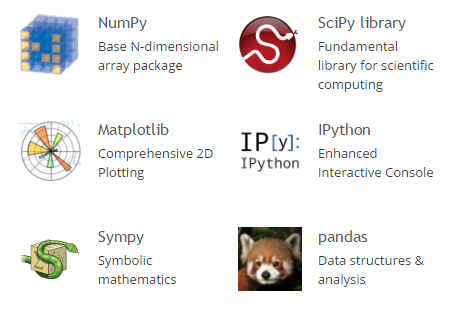
\includegraphics[width=0.75\linewidth]{fig/scipy.png}}



% !split
\subsection{Arrays}
\label{sec:arrays}

Numpy arrays are similar to lists, but can only contain one datatype, but capable of N-dimensional arrays(or matrices) . Arrays and are optimized for numerics and linear algebra. Arrays are around 30x faster than lists.

\emph{Note} - numpy does have a matrix class which was designed for linear algebra, but it is recommended to use the array class to avoid confusion when performing calculations.

\begin{Verbatim}[numbers=none,fontsize=\fontsize{9pt}{9pt},baselinestretch=0.95,xleftmargin=2mm]
# make sure to import the functions you need
from numpy import array, arange, linspace, sin
# If you need more functions, import the whole module
import numpy as np

# using the range function to create a numpy array
x = array(range(10))
print('x = ',x, 'as a',x.dtype)
\end{Verbatim}

% !bpop
\begin{Verbatim}[numbers=none,fontsize=\fontsize{9pt}{9pt},baselinestretch=0.95,xleftmargin=2mm]
x =  [0 1 2 3 4 5 6 7 8 9] as a int64
\end{Verbatim}
% !epop

\begin{Verbatim}[numbers=none,fontsize=\fontsize{9pt}{9pt},baselinestretch=0.95,xleftmargin=2mm]
# using numpy function arange
x = arange(10)
print('x = ',x, 'as a',x.dtype)
\end{Verbatim}

% !bpop
\begin{Verbatim}[numbers=none,fontsize=\fontsize{9pt}{9pt},baselinestretch=0.95,xleftmargin=2mm]
x =  [0 1 2 3 4 5 6 7 8 9] as a int64
\end{Verbatim}
% !epop

\begin{Verbatim}[numbers=none,fontsize=\fontsize{9pt}{9pt},baselinestretch=0.95,xleftmargin=2mm]
# numpy array
x = linspace(0,9,10)
print('x = ',x, 'as a',x.dtype)
\end{Verbatim}

% !bpop
\begin{Verbatim}[numbers=none,fontsize=\fontsize{9pt}{9pt},baselinestretch=0.95,xleftmargin=2mm]
x =  [ 0.  1.  2.  3.  4.  5.  6.  7.  8.  9.] as a float64
\end{Verbatim}
% !epop

% !split
\subsection{Array Operations}

Element-wise operations
\begin{Verbatim}[numbers=none,fontsize=\fontsize{9pt}{9pt},baselinestretch=0.95,xleftmargin=2mm]
# element-wise array multiplcation
x*3
\end{Verbatim}


% !bpop
\begin{Verbatim}[numbers=none,fontsize=\fontsize{9pt}{9pt},baselinestretch=0.95,xleftmargin=2mm]
array([  0.,   3.,   6.,   9.,  12.,  15.,  18.,  21.,  24.,  27.])
\end{Verbatim}
% !epop


\begin{Verbatim}[numbers=none,fontsize=\fontsize{9pt}{9pt},baselinestretch=0.95,xleftmargin=2mm]
# element-wise array exponentiation
x**2
\end{Verbatim}

% !bpop
\begin{Verbatim}[numbers=none,fontsize=\fontsize{9pt}{9pt},baselinestretch=0.95,xleftmargin=2mm]
array([  0.,   1.,   4.,   9.,  16.,  25.,  36.,  49.,  64.,  81.])
\end{Verbatim}
% !epop


% element-wise array trigonometry functions
\begin{Verbatim}[numbers=none,fontsize=\fontsize{9pt}{9pt},baselinestretch=0.95,xleftmargin=2mm]
sin(x)
\end{Verbatim}

% !bpop
\begin{Verbatim}[numbers=none,fontsize=\fontsize{9pt}{9pt},baselinestretch=0.95,xleftmargin=2mm]
array([ 0.        ,  0.84147098,  0.90929743,  0.14112001, -0.7568025 ,    -0.95892427, -0.2794155 ,  0.6569866 ,  0.98935825,  0.41211849])
\end{Verbatim}
% !epop


% !split
\subsection{Array Operations}

Often, objects in python have many methods that can be performed on that data-type. To see what methods are available, a \texttt{.} can be typed to see what is available or the \texttt{dir()} function can be used

\begin{Verbatim}[numbers=none,fontsize=\fontsize{9pt}{9pt},baselinestretch=0.95,xleftmargin=2mm]
# show all methods available for variable/object x
print([k for k in dir(x) if k[:2] != '__' ])
\end{Verbatim}

% !bpop
\begin{Verbatim}[numbers=none,fontsize=\fontsize{9pt}{9pt},baselinestretch=0.95,xleftmargin=2mm]
['T', 'all', 'any', 'argmax', 'argmin', 'argpartition', 'argsort',\ 'astype', 'base', 'byteswap', 'choose', 'clip', 'compress', 'conj',\ 'conjugate', 'copy', 'ctypes', 'cumprod', 'cumsum', 'data', 'diagonal',\ 'dot', 'dtype', 'dump', 'dumps', 'fill', 'flags', 'flat', 'flatten',\ 'getfield', 'imag', 'item', 'itemset', 'itemsize', 'max', 'mean', 'min',\ 'nbytes', 'ndim', 'newbyteorder', 'nonzero', 'partition', 'prod', 'ptp',\ 'put', 'ravel', 'real', 'repeat', 'reshape', 'resize', 'round',\ 'searchsorted', 'setfield', 'setflags', 'shape', 'size', 'sort',\ 'squeeze', 'std', 'strides', 'sum', 'swapaxes', 'take', 'tobytes',\ 'tofile', 'tolist', 'tostring', 'trace', 'transpose', 'var', 'view']
\end{Verbatim}
% !epop

% array methods
\begin{Verbatim}[numbers=none,fontsize=\fontsize{9pt}{9pt},baselinestretch=0.95,xleftmargin=2mm]
# using method sum for variable x
x.sum()
# also use the sum function from the numpy module
np.sum(x)
\end{Verbatim}

% !bpop
\begin{Verbatim}[numbers=none,fontsize=\fontsize{9pt}{9pt},baselinestretch=0.95,xleftmargin=2mm]
45
\end{Verbatim}
% !epop


% !split
\subsection{Logical Indexing}

A powerful filtering technique in Matlab and python called logical indexing is a great way to perform calculations to specific numbers or filter data

\begin{Verbatim}[numbers=none,fontsize=\fontsize{9pt}{9pt},baselinestretch=0.95,xleftmargin=2mm]
# logical indexing
3 < x
\end{Verbatim}

% !bpop
\begin{Verbatim}[numbers=none,fontsize=\fontsize{9pt}{9pt},baselinestretch=0.95,xleftmargin=2mm]
array([False, False, False, False,  True,  True,  True,  True,  True,  True], dtype=bool)
\end{Verbatim}
% !epop

\begin{Verbatim}[numbers=none,fontsize=\fontsize{9pt}{9pt},baselinestretch=0.95,xleftmargin=2mm]
# negate logical index
~(3 < x)
\end{Verbatim}

% !bpop
\begin{Verbatim}[numbers=none,fontsize=\fontsize{9pt}{9pt},baselinestretch=0.95,xleftmargin=2mm]
array([ True,  True,  True,  True, False, False, False, False, False, False], dtype=bool)
\end{Verbatim}
% !epop

\begin{Verbatim}[numbers=none,fontsize=\fontsize{9pt}{9pt},baselinestretch=0.95,xleftmargin=2mm]
# and logical index operator
(3 < x) & (x < 5)
\end{Verbatim}

% !bpop
\begin{Verbatim}[numbers=none,fontsize=\fontsize{9pt}{9pt},baselinestretch=0.95,xleftmargin=2mm]
array([False, False, False, False,  True, False, False, False, False, False], dtype=bool)
\end{Verbatim}
% !epop

\begin{Verbatim}[numbers=none,fontsize=\fontsize{9pt}{9pt},baselinestretch=0.95,xleftmargin=2mm]
# or logical index operator
(3 < x) | (x < 5)
\end{Verbatim}

% !bpop
\begin{Verbatim}[numbers=none,fontsize=\fontsize{9pt}{9pt},baselinestretch=0.95,xleftmargin=2mm]
array([ True,  True,  True,  True,  True,  True,  True,  True,  True,  True], dtype=bool)
\end{Verbatim}
% !epop

\begin{Verbatim}[numbers=none,fontsize=\fontsize{9pt}{9pt},baselinestretch=0.95,xleftmargin=2mm]
# multiple and logical index operator
(3 < x) & (x < 5)
\end{Verbatim}

% !bpop
\begin{Verbatim}[numbers=none,fontsize=\fontsize{9pt}{9pt},baselinestretch=0.95,xleftmargin=2mm]
array([False, False, False, False,  True, False, False, False, False, False], dtype=bool)
\end{Verbatim}
% !epop

% !split
\subsection{Multi-Dimensional Arrays (matrices)}

Numpy has both array classes and a matrix class. The array is a more general object, where the matrix class is specifically for linear algebra. Matrices are only 2-dimensional, which can limit functionality, where the array can be n-dimensional. All matrix operations can be performed on an array, so it is recommended to just use arrays to avoid confusion.

First, to define a 1x3 array
\begin{Verbatim}[numbers=none,fontsize=\fontsize{9pt}{9pt},baselinestretch=0.95,xleftmargin=2mm]
c = array([[1,2,3]])
c
\end{Verbatim}

% !bpop
\begin{Verbatim}[numbers=none,fontsize=\fontsize{9pt}{9pt},baselinestretch=0.95,xleftmargin=2mm]
array([[1, 2, 3]])
\end{Verbatim}
% !epop


Now the transpose does what we expected to a 3x1 array
\begin{Verbatim}[numbers=none,fontsize=\fontsize{9pt}{9pt},baselinestretch=0.95,xleftmargin=2mm]
c.transpose()
\end{Verbatim}

% !bpop
\begin{Verbatim}[numbers=none,fontsize=\fontsize{9pt}{9pt},baselinestretch=0.95,xleftmargin=2mm]
array([[1],
       [2],
       [3]])
\end{Verbatim}
% !epop

If we want to define a 3x1 array, we define the array like so
\begin{Verbatim}[numbers=none,fontsize=\fontsize{9pt}{9pt},baselinestretch=0.95,xleftmargin=2mm]
c = array( [[1],[2],[3]] )
\end{Verbatim}

% !bpop
\begin{Verbatim}[numbers=none,fontsize=\fontsize{9pt}{9pt},baselinestretch=0.95,xleftmargin=2mm]
array([[1],
       [2],
       [3]])
\end{Verbatim}
% !epop

% !split
\subsection{Matrix Pitfalls}

Defining an array is simple but if you are used to Matlab syntax, there could be some confusion. In Matlab, every array(or vector) is at least a (1,1). In python, it is possible to define a (3,), which can be very frustrating if, for example you are interested in transposing your array from a row to a column. Lets take a look.

\begin{Verbatim}[numbers=none,fontsize=\fontsize{9pt}{9pt},baselinestretch=0.95,xleftmargin=2mm]
# create a 3 element array
c = array([1,2,3])
c
\end{Verbatim}

% !bpop
\begin{Verbatim}[numbers=none,fontsize=\fontsize{9pt}{9pt},baselinestretch=0.95,xleftmargin=2mm]
array([1, 2, 3])
\end{Verbatim}
% !epop

\begin{Verbatim}[numbers=none,fontsize=\fontsize{9pt}{9pt},baselinestretch=0.95,xleftmargin=2mm]
c.transpose()
\end{Verbatim}

% !bpop
\begin{Verbatim}[numbers=none,fontsize=\fontsize{9pt}{9pt},baselinestretch=0.95,xleftmargin=2mm]
array([1, 2, 3])
\end{Verbatim}
% !epop

That is not what I expected. I thought it would be a column array not, but no.~Upon further inspection, welcome to the (3,) dimension array.

\begin{Verbatim}[numbers=none,fontsize=\fontsize{9pt}{9pt},baselinestretch=0.95,xleftmargin=2mm]
c.shape
\end{Verbatim}

% !bpop
\begin{Verbatim}[numbers=none,fontsize=\fontsize{9pt}{9pt},baselinestretch=0.95,xleftmargin=2mm]
(3,)
\end{Verbatim}
% !epop

This can be addressed in a few ways. The safest solution is to change how the arrays are defined.

% !split
\subsection{Matrix Operations}

lets creat some matrices (but recall use the array)

\begin{Verbatim}[numbers=none,fontsize=\fontsize{9pt}{9pt},baselinestretch=0.95,xleftmargin=2mm]
a = array([[1, 2], [3, 4]])
a
\end{Verbatim}

% !bpop
\begin{Verbatim}[numbers=none,fontsize=\fontsize{9pt}{9pt},baselinestretch=0.95,xleftmargin=2mm]
array([[1, 2],
       [3, 4]])
\end{Verbatim}
% !epop

\begin{Verbatim}[numbers=none,fontsize=\fontsize{9pt}{9pt},baselinestretch=0.95,xleftmargin=2mm]
b = array([[1, 2, 4],[5, 6, 7] ])
b
\end{Verbatim}

% !bpop
\begin{Verbatim}[numbers=none,fontsize=\fontsize{9pt}{9pt},baselinestretch=0.95,xleftmargin=2mm]
array([[1, 2, 4],
       [5, 6, 7]])
\end{Verbatim}
% !epop

To perform a matrix multiplication on an array, use the \texttt{@}

\begin{Verbatim}[numbers=none,fontsize=\fontsize{9pt}{9pt},baselinestretch=0.95,xleftmargin=2mm]
a @ b
\end{Verbatim}

% !bpop
\begin{Verbatim}[numbers=none,fontsize=\fontsize{9pt}{9pt},baselinestretch=0.95,xleftmargin=2mm]
array([[11, 14, 18],
       [23, 30, 40]])
\end{Verbatim}
% !epop

To perform element wise operation, use \texttt{*}

\begin{Verbatim}[numbers=none,fontsize=\fontsize{9pt}{9pt},baselinestretch=0.95,xleftmargin=2mm]
b * 27
\end{Verbatim}

% !bpop
\begin{Verbatim}[numbers=none,fontsize=\fontsize{9pt}{9pt},baselinestretch=0.95,xleftmargin=2mm]
array([[ 27,  54, 108],
       [135, 162, 189]])
\end{Verbatim}
% !epop


% !split
\subsection{Plotting}

Finally, to wrap up this scientific computing tutorial, we end with plotting. Sometimes it is difficult to communicate a calculation or understand complex datasets. Graphs and Plots are such an important part of science and engineering that the python science stack comes with a powerful yet simple plotting packaged called \emph{matplotlib}. Plotting can be just as complicated as the calculations, so here is a simple example to get started. Check out the \href{{http://matplotlib.org/gallery.html}}{matplotlib gallery} for many more examples.

\begin{Verbatim}[numbers=none,fontsize=\fontsize{9pt}{9pt},baselinestretch=0.95,xleftmargin=2mm]
from numpy import *
from matplotlib.pyplot import *
x = linspace(-20,20,100)
plot(x,sin(x)/x)
title('y=sin(x)/x')
savefig('fig/matplotlib.png')
show()
\end{Verbatim}



% inline figure
\centerline{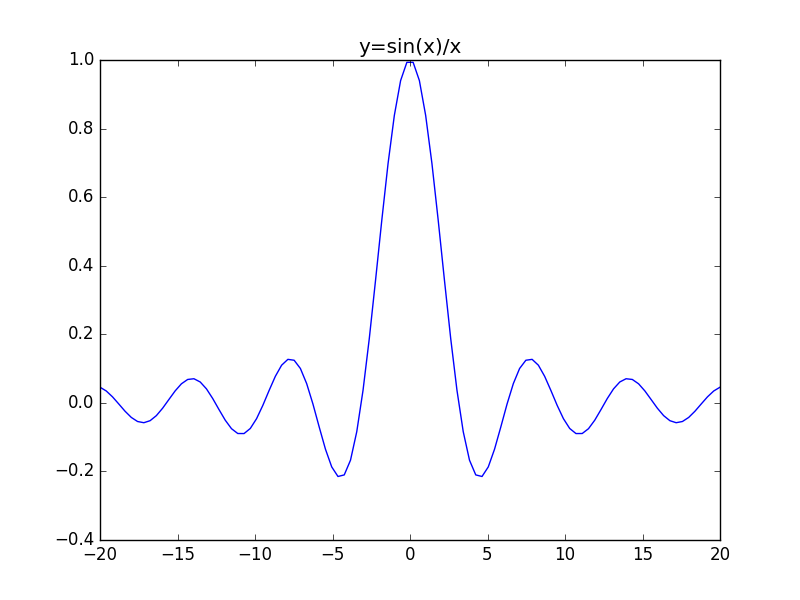
\includegraphics[width=0.9\linewidth]{fig/matplotlib.png}}




% !split
\subsection{Python in Engineering Summary}

A brief introduction to the python programming language has been presented to demonstrate the capabilities of python for scientific computing applied to physics and engineering. If your curiosity got the better part of you, please check out the following links that I have found very useful in the (\ref{sec:reflinks}) section.


% !split
\subsection{References and Links}
\label{sec:reflinks}


\paragraph{MATLAB vs Python.}
Other comparisons of python versus MATLAB  \\
\href{{http://fperez.org/py4science/warts.html}}{\nolinkurl{http://fperez.org/py4science/warts.html}} \\
\href{{http://www.pyzo.org/whypython.html}}{\nolinkurl{http://www.pyzo.org/whypython.html}} \\
\href{{http://www.pyzo.org/python_vs_matlab.html}}{\nolinkurl{http://www.pyzo.org/python_vs_matlab.html}} \\
\href{{https://www.mathworks.com/products/matlab/matlab-vs-python.html#comparison_table}}{\nolinkurl{https://www.mathworks.com/products/matlab/matlab-vs-python.html\#comparison_table}} \\
\href{{https://docs.scipy.org/doc/numpy-dev/user/numpy-for-matlab-users.html}}{\nolinkurl{https://docs.scipy.org/doc/numpy-dev/user/numpy-for-matlab-users.html}} \\



\paragraph{Python Syntax Cheatsheets.}
\href{{https://damontallen.github.io/IPython-quick-ref-sheets/}}{ipython-chetasheet} \\
\href{{http://conda.pydata.org/docs/using/cheatsheet.html}}{conda-chetasheet} \\
\href{{http://mathesaurus.sourceforge.net/matlab-numpy.html}}{python for matlab users} \\


% !split
\paragraph{Python Engineering Books.}
\href{{http://www.apress.com/9781484205549}}{Numerical Python - A Practical Techniques Approach for Industry} with \href{{http://www.apress.com/downloadable/download/sample/sample_id/1732/}}{source code}  \\
\href{{http://www.springer.com/us/book/9783319195957#aboutBook}}{Elementary Mechanics Using Python}   \\
\href{{http://hplgit.github.io/primer.html/doc/web/index.html}}{A Primer on Scientific Programming With Python}  \\
\href{{http://codingthematrix.com/}}{Coding the Matrix} \\
\href{{http://www.springer.com/us/book/9783540739159}}{Python Scripting for Computational Science} \\
\href{{http://www.springer.com/us/book/9783662498866}}{A Primer on Scientific Programming with Python}  with \href{{https://hplgit.github.io/primer.html/doc/pub/half/book.pdf}}{partial free download} \\
\href{{http://www-personal.umich.edu/~mejn/computational-physics/}}{Computation Physics} \\

\paragraph{Python Engineering Library Documentation.}
Python has mature scientific computation packages, namely \href{{https://www.scipy.org/}}{scipy} \\

\textbf{Scipy}.

\href{{http://scipy-cookbook.readthedocs.io/index.html}}{Scipy Cookbook}  \\
\href{{http://www.davekuhlman.org/scipy_guide_01.html}}{Scipy Guide}  \\
\href{{http://www.scipy-lectures.org/index.html}}{Scipy Lectures}   \\
\href{{https://github.com/rojassergio/Learning-Scipy}}{Learning Scipy}   \\
\href{{http://docs.scipy.org/doc/scipy/reference/tutorial/}}{Scipy Tutorial}   \\

\textbf{Numpy}.

\href{{https://wiki.python.org/moin/NumericAndScientific}}{Numpy}  \\
\href{{https://docs.scipy.org/doc/numpy-dev/contents.html}}{Official Docs}  \\
\href{{https://docs.scipy.org/doc/numpy-dev/user/numpy-for-matlab-users.html}}{Numpy for matlab users}  \\
\href{{https://github.com/rougier/numpy-100}}{100 numpy examples}  \\
\href{{https://github.com/numpy/numpy/wiki/Numerical-software-on-Windows}}{numpy on windows}  \\

\textbf{Sympy}.

\href{{http://docs.sympy.org/dev/tutorial/intro.html}}{sympy tutorial} \\
\href{{http://www.sympy.org/en/features.html}}{sympy features} \\
\href{{http://docs.sympy.org/dev/modules/physics/mechanics/}}{sympy physics} \\

\textbf{Matplotlib}.

\href{{http://matplotlib.org/gallery.html}}{matplotlib gallery} and \href{{https://github.com/rougier/matplotlib-tutorial}}{matplotlib tutorial}  \\
\href{{http://central.scipy.org/item/84/1/simple-interactive-matplotlib-plots}}{interactive matplotlib} \\

% !split
\paragraph{General Python.}
\href{{http://docs.python-guide.org/en/latest/}}{The Hitchhikers Guide to Python} \\
\href{{http://hplgit.github.io/bumpy/doc/pub/._basics000.html#table_of_contents}}{A very basic introduction to scientific Python programming}  \\

\paragraph{Python and Excel Spreadsheets.}
\href{{http://www.xlwings.org}}{xlwings} \\
\href{{http://pandas.pydata.org}}{pandas} \\

\paragraph{Python Online Courses.}
\href{{https://github.com/jrjohansson/scientific-python-lectures}}{scientific-python-lectures}  \\
\href{{http://openedx.seas.gwu.edu/courses/GW/MAE6286/2014_fall/about}}{Practical Numerical Methods with Python} with \href{{https://github.com/numerical-mooc/numerical-mooc}}{source code} \\
\href{{http://openedx.seas.gwu.edu/courses/GW/MAE6226/2014_spring/about}}{Aerodynamics / Hydrodynamics with Python} \\
\href{{http://pages.physics.cornell.edu/~sethna/StatMech/ComputerExercises/PythonSoftware/}}{Cornell}  \\
\href{{http://openedx.seas.gwu.edu/courses/GW/MAE6286/2014_fall/about}}{Python numerical methods mooc}  \\
\href{{http://www-personal.umich.edu/~mejn/computational-physics/}}{Computational Physics with Python} \\
\href{{http://cs.brown.edu/courses/cs053/current/index.htm}}{Coding the Matrix} \\
\href{{http://interactivepython.org/runestone/static/thinkcspy/index.html}}{How to Think Like a Computer Scientist} \\

\paragraph{Programming Games.}
\href{{https://projecteuler.net/}}{project euler} \\
\href{{https://checkio.org/}}{checkio} \\
\href{{https://github.com/rougier/numpy-100/blob/master/100%20Numpy%20exercises.md}}{Numeric Python exercises} \\




\vspace{3mm}




\vspace{3mm}



% ------------------- end of main content ---------------


% #ifdef PREAMBLE

\printindex

\end{document}
% #endif

